\section{Anatomical recovery and measurement validity}
\label{sec:validity}

Sections~\ref{sec:framework} and~\ref{sec:algo} established what the objective
observes and what each mechanism adds. This section asks what the recovered
representation supports as a measurement, using the vocabulary that the experiments
force. \emph{Geometric agreement}: the surfaces overlap. \emph{Surface
correspondence}: points are mapped geometrically. \emph{Anatomical correspondence}:
the mapping preserves anatomical identity. \emph{Parametric recovery}: the recovered
$\bm\beta,\bm\theta$ have a stable meaning across specimens. \emph{Measurement
validity}: a quantity extracted from those parameters agrees with a reference. Each
level is necessary for the next and none implies it.

\subsection{Surface agreement versus anatomical correctness}
\label{sec:geometric-agreement}

\textbf{Question and test.} If a fit scores better on the objective's own terms, is
its skeleton better? Within the Joint Alignment Benchmark, the free-form deformation
and normal regularisation were removed from the production recipe, and surface and
skeleton were compared across twelve strategies. \textbf{Finding.} This produced the
\emph{closest} surface of all twelve strategies (about $0.45\times$ the Chamfer
distance) and one of the worst skeletons (joint-level ratio $1.25$, worse on 8 of 11
specimens), and no strategy lay in the quadrant of better surface \emph{and} better
skeleton (Figure~\ref{fig:dissociation}). Removing the regularisation inflated the
free-form deformation roughly nine-fold: the surface was fitted by moving the skin
and not the skeleton, which is the prediction of Equation~\eqref{eq:gauge}. The
joint-level model resolves the effect, and the specimen-level test, whose threshold
is about ten of eleven consistent specimens, shows the same direction on eight.

\textbf{Implication.} Surface agreement can certify coverage of the scan and nothing
about anatomical identity, so a surface metric must not be used to choose a method
for anatomical accuracy. The dissociation of fit error from target error is
established in registration more generally~\cite{fitzpatrick}; what the benchmark
adds is its measured size in a deformable articulated model, under a pre-registered
single-factor ablation, together with the adversarial demonstration of
Section~\ref{sec:protocol}.

\begin{figure}[!htb]
\centering
\begin{minipage}[b]{0.46\linewidth}
\centering
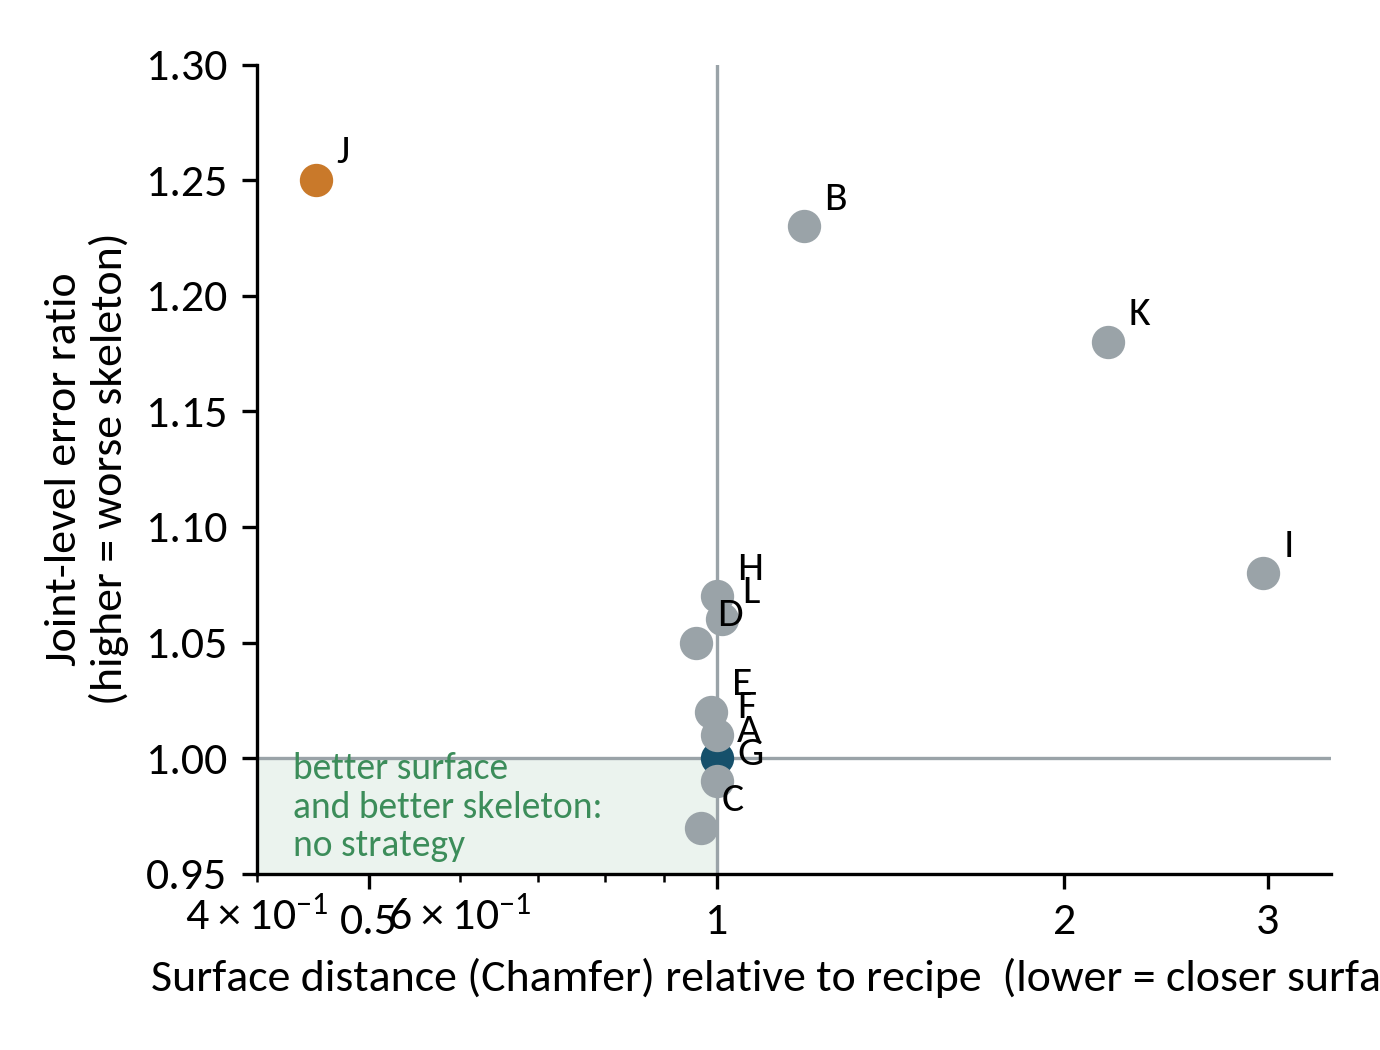
\includegraphics[width=\linewidth]{figures/fig_dissociation.png}
\end{minipage}\hfill
\begin{minipage}[b]{0.48\linewidth}
\centering
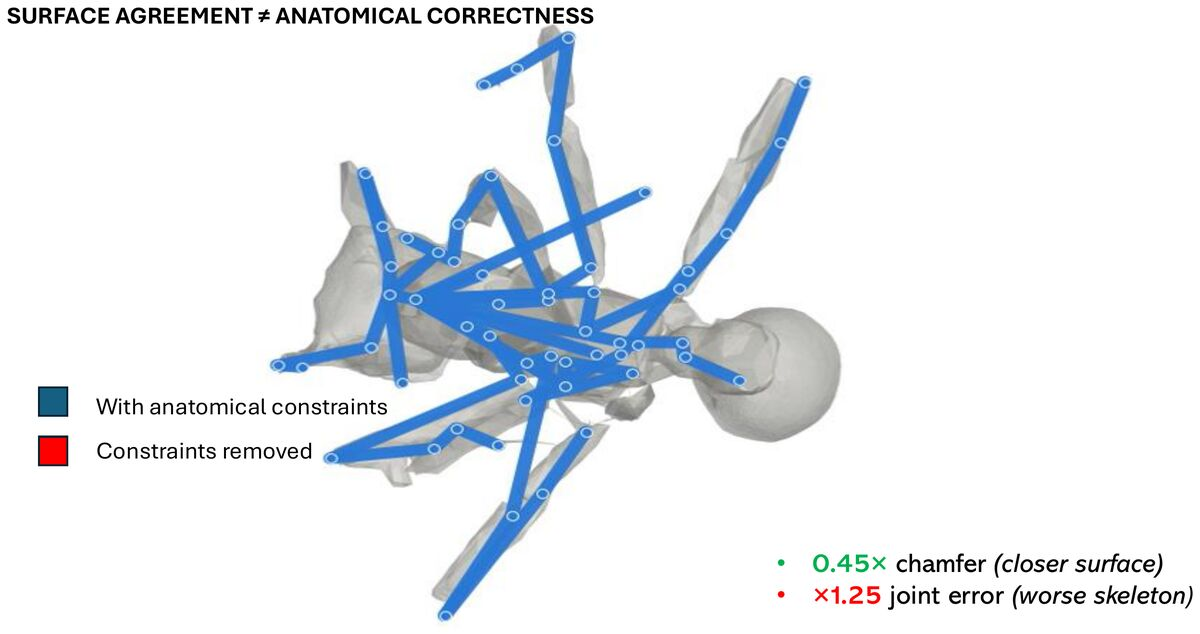
\includegraphics[width=\linewidth]{figures/fig_geometric_agreement.jpg}
\end{minipage}
\caption[Surface agreement and anatomical correctness]{Left: surface distance against
skeleton error across the twelve strategies (letters as in Figure~\ref{fig:jab}); the
strategy with the closest surface, J, has one of the worst skeletons, and none improves
both. Right: the skeleton overlay with the regularisation active; removing it yields a
closer surface and a worse skeleton.}
\label{fig:dissociation}
\end{figure}

\subsection{Skeleton recovery against the expert reference}
\label{sec:skeleton}

\textbf{What the objective observes, and what the output requires.} The objective
observes surface geometry, normals, mesh regularity, symmetry and rotation ranges.
The desired output additionally requires joint location, anatomical identity and
within-structure correspondence. No term of the objective explicitly observes joint
position, and reweighting an existing term cannot recover information that the
objective does not observe. The benchmark tests this directly.

\textbf{Evidence.} Production joint error is about a quarter of Weber's length (median
$25.1\%$, 95\% CI $17.5$--$44.8$). Supplying expert joint targets during fitting lowers
the error to $17.4\%$, from $26.9\%$ in a paired control that re-fits the same specimens
without targets ($10$ of $11$ improve; the control itself leaves the error unchanged), so a
better skeleton exists within the model's own shape budget. Yet no single-factor change
to the recipe improves joint alignment reliably, and the recipe ranks best of the
twelve (Figure~\ref{fig:jab}, left). Supervision supplied for every region
\emph{except} one leaves that region essentially unchanged, with every held-out
interval including zero: supervision acts locally and does not propagate. Alignment is
largely won in a single place, the part-wise leg stage, which improved all eleven
specimens, while later steps add little (Figure~\ref{fig:jab}, right); the scale
regularisation and the allometric prior are joint-neutral.

\begin{figure}[!htb]
\centering
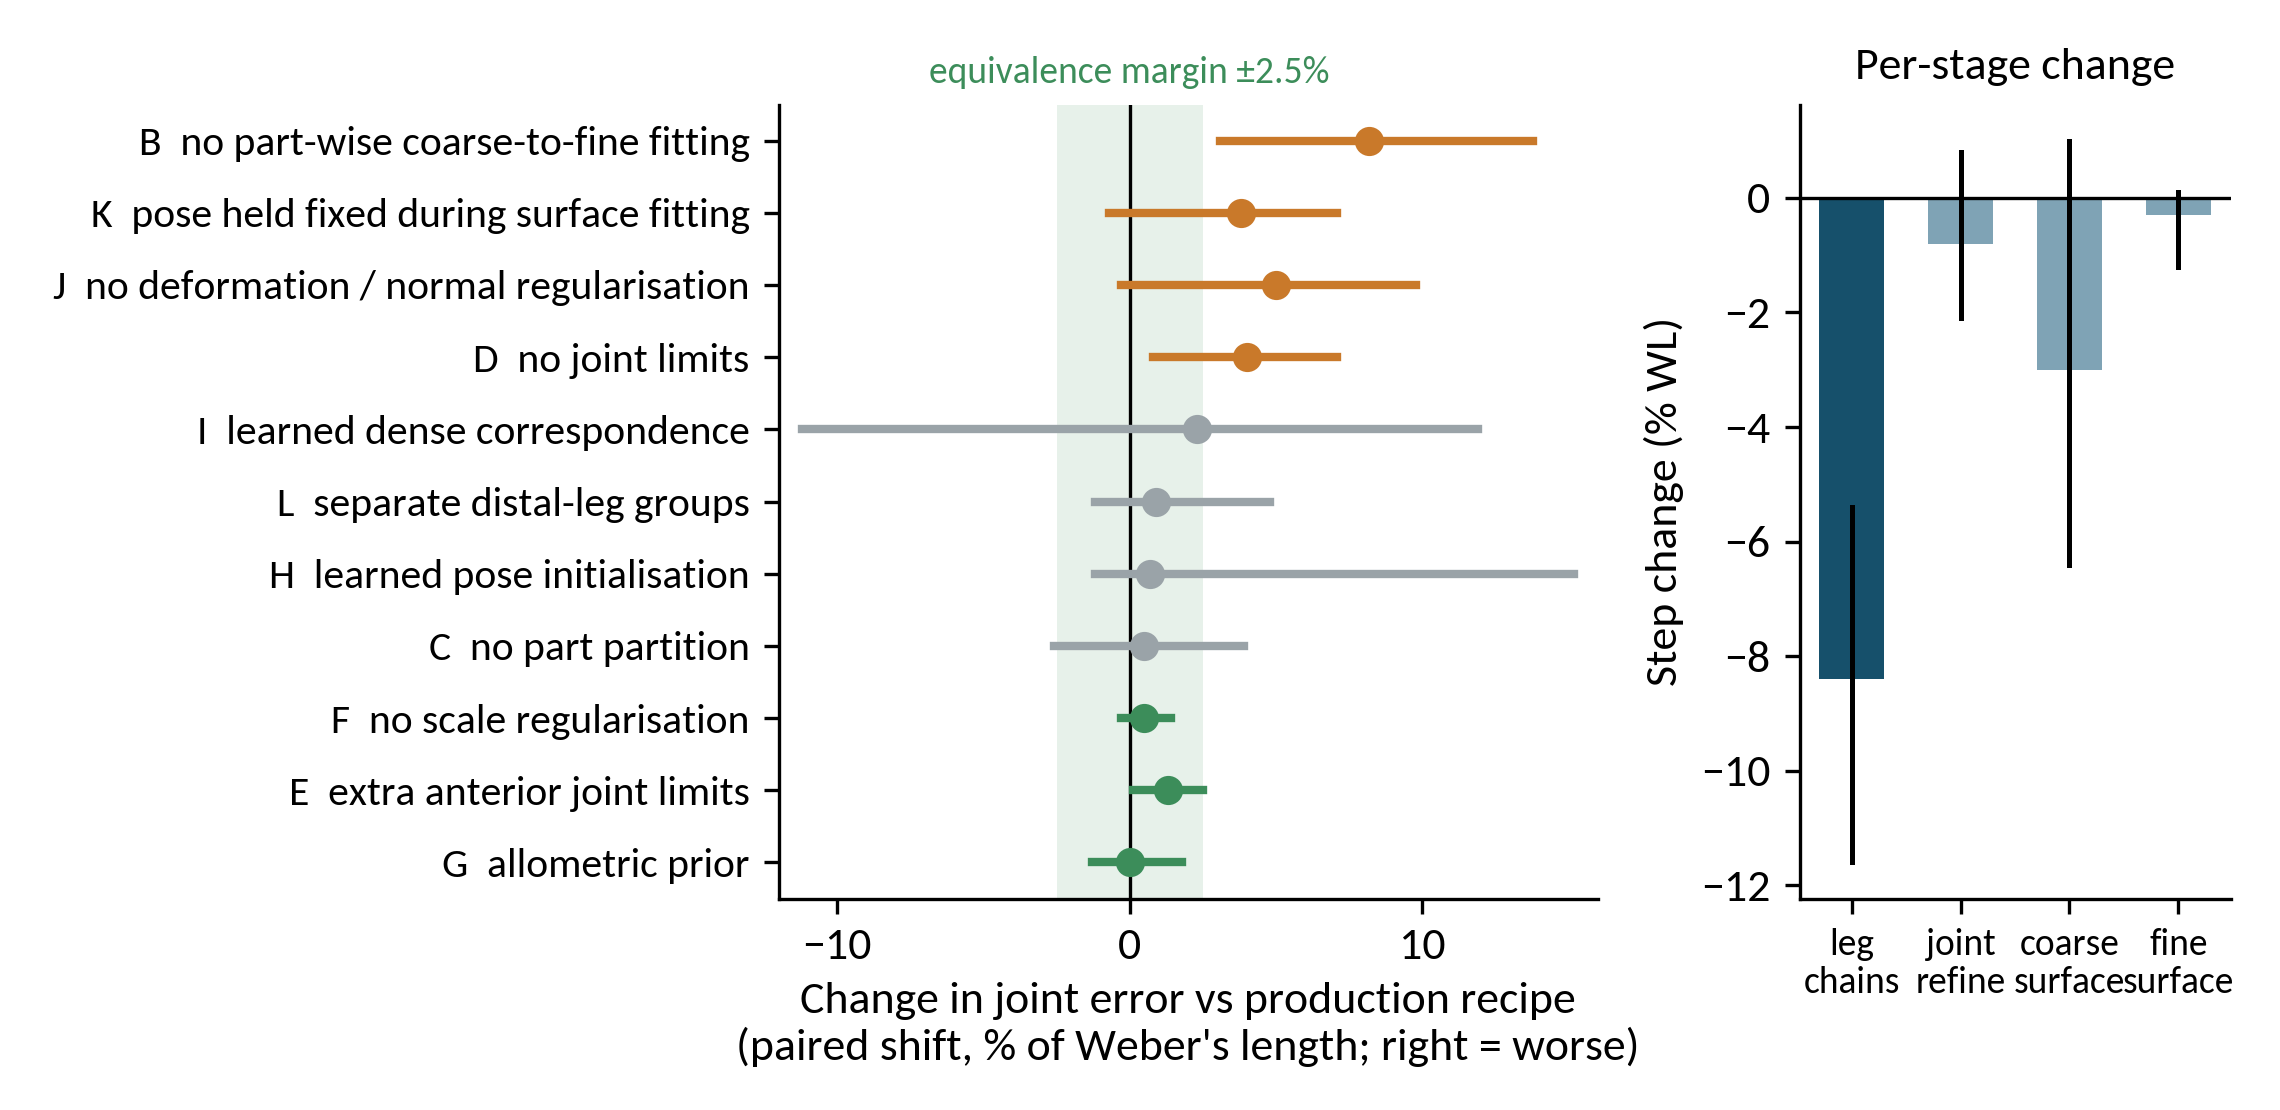
\includegraphics[width=0.78\linewidth]{figures/fig_jab_contrasts.png}
\caption[Joint Alignment Benchmark]{Joint Alignment Benchmark ($n=11$ specimens, 396
fits). Left: paired change in joint error for each single-factor strategy against the
production recipe, with 95\% intervals; the shaded band is the $\pm2.5\%$ equivalence
margin, and green marks strategies equivalent to the recipe. Right: per-stage change in
joint error within the recipe.}
\label{fig:jab}
\end{figure}

\textbf{Structure of the error.} The error is not uniform
(Figure~\ref{fig:structured-error}): proximal leg joints are placed at about
$12$--$13\%$ of WL, the body axis at $24\%$, and the mandibles, antennae and thin
distal segments at $43$--$56\%$. A variance decomposition attributes far more of the
spread to \emph{which joint} and \emph{which specimen} than to the optimiser seed, so
the failure is anatomically structured. The ordering is the expected one, since pose
estimation has long reported error growing along a kinematic chain; what the benchmark
supplies is the usable per-region number.

\begin{figure}[!htb]
\centering
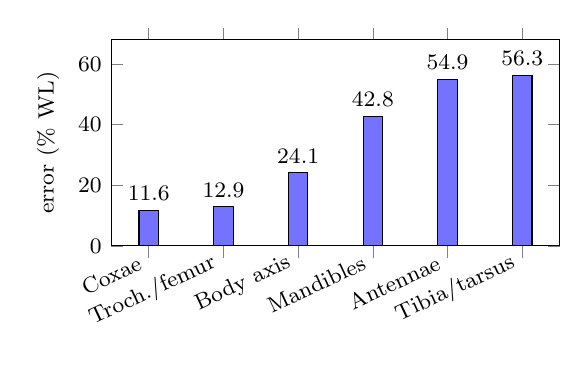
\begin{tikzpicture}
\begin{axis}[ybar,width=0.60\linewidth,height=4.2cm,bar width=7pt,ymin=0,ymax=68,
 symbolic x coords={Coxae,Troch./femur,Body axis,Mandibles,Antennae,Tibia/tarsus},
 xtick=data,x tick label style={rotate=25,anchor=east,font=\footnotesize},
 ylabel={error (\% WL)},ylabel style={font=\footnotesize},tick label style={font=\footnotesize},
 nodes near coords,every node near coord/.append style={font=\footnotesize}]
\addplot[fill=blue!55] coordinates {(Coxae,11.6)(Troch./femur,12.9)(Body axis,24.1)(Mandibles,42.8)(Antennae,54.9)(Tibia/tarsus,56.3)};
\end{axis}
\end{tikzpicture}
\hfill
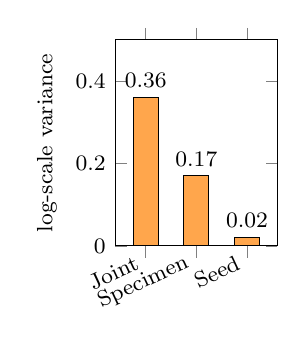
\begin{tikzpicture}
\begin{axis}[ybar,width=0.30\linewidth,height=4.2cm,bar width=9pt,ymin=0,ymax=0.5,
 enlarge x limits=0.3,
 symbolic x coords={Joint,Specimen,Seed},xtick=data,tick label style={font=\footnotesize},
 x tick label style={rotate=25,anchor=east},
 ylabel={log-scale variance},ylabel style={font=\footnotesize},nodes near coords,
 every node near coord/.append style={font=\footnotesize,/pgf/number format/fixed,/pgf/number format/precision=2}]
\addplot[fill=orange!70] coordinates {(Joint,0.36)(Specimen,0.17)(Seed,0.02)};
\end{axis}
\end{tikzpicture}
\caption[Structure of the skeleton error]{Left: median skeleton error by region for the
production recipe. Right: variance decomposition across the same fits; the optimiser seed
contributes almost nothing.}
\label{fig:structured-error}
\end{figure}

\subsection{From recovered parameters to measurable traits}
\label{sec:measurement}

A number extracted from an articulated fitted model is not automatically a
morphometric. Four validity axes fail independently, which is why one is not enough: the
trait's endpoints sit on the structure it is named after (\emph{anatomical}); it is stable
when only the articulation changes (\emph{pose invariance}); it reproduces a known scaling
relationship (\emph{biological}); and it is internally consistent, for instance in its
bilateral asymmetry, since near-symmetric animals make left--right disagreement a
measure of error (\emph{consistency}). A trait can be perfectly pose-stable and still be
anatomically wrong, measuring the wrong structure consistently, so any single axis can
certify a fit that is wrong. The internal-consistency axis ranks traits correctly but is a
trait-level screen and not a per-specimen confidence score, because within a trait
asymmetry does not predict pose contamination.

Manual joint annotation by an expert (Figure~\ref{fig:ground-truth}) provides the reference
for the skeleton-based axes. Head width, read from two reporter bones placed on the head
capsule, is the trait that carries this validation. It is the most pose-invariant trait examined (its value changes by
about $0.1\%$ when only articulation changes), its endpoints are defined by a part extent
and not by landmark indices, and it reproduces the allometric scaling of head width against
body length (exponent $1.21$, interval $1.15$--$1.26$, against $1.24$ in the reference
data). Against the reference head widths supplied with the \emph{Atta vollenweideri} data
set for 20 workers, the mean absolute difference is about $4\%$
(Figure~\ref{fig:head-width}). Agreement in millimetres is partly shared with the
reference because scale is restored from body length, so the dimensionless ratio of head
width to body length is the informative test; it also agrees (concordance coefficient
$0.86$; the mean relative difference is the same as for the absolute value by
construction, since body length cancels, so the informative change is the fall in
concordance once the shared size is removed), with a modest size-dependent bias that is the same effect as the slightly
compressed scaling exponent: the model slightly compresses the allometric relationship at
the extremes of the size range. The two head-width definitions tested are not
interchangeable (the reporter-bone distance is essentially unbiased, whereas a
Type~III extent carries a systematic $+2\%$ bias), so the definition is part of the
measurement.

\begin{figure}[!htb]
\centering
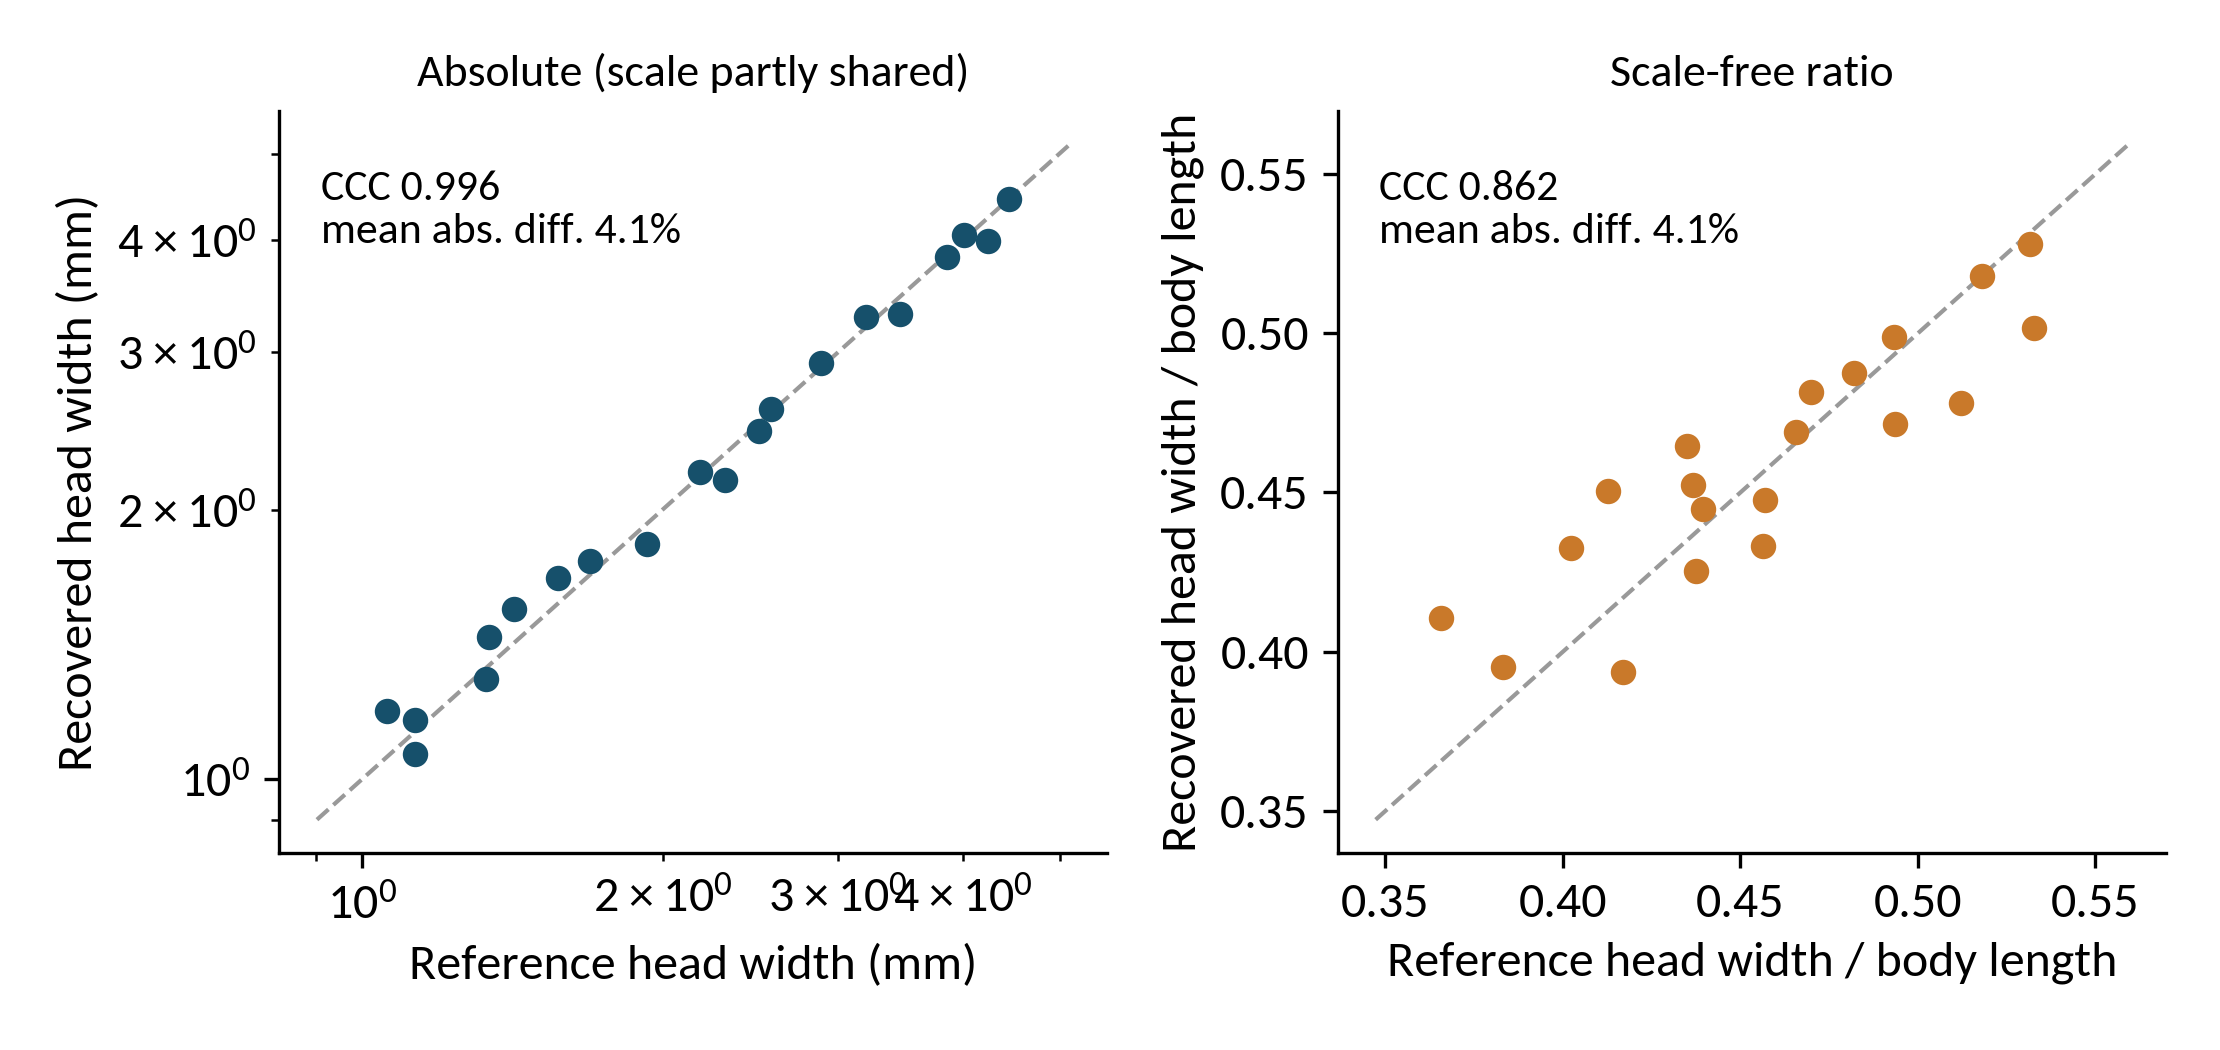
\includegraphics[width=0.62\linewidth]{figures/fig_head_width_agreement.png}
\caption[Head-width agreement]{Head width recovered by the registration against the reference
table supplied with the data set (20 \emph{Atta vollenweideri} workers). Left: absolute head
width (log scale; scale is partly shared through body length). Right: scale-free ratio of
head width to body length, the independent test; the mean relative difference is
identical to the left panel by construction (body length cancels), whereas concordance
falls from $0.996$ to $0.86$. Dashed lines are identity.}
\label{fig:head-width}
\end{figure}

The same framework identifies where measurement should not be trusted. Traits whose
endpoints are rig pivots instead of surface-defined points, or that are sensitive to
articulation, require a different definition before use. Registration of an independent
ethanol-preserved worker corpus sits at a measurable noise floor, at which two conspecific
workers are only about $7\%$ closer than unrelated ants, and distal leg and antenna segment
lengths, the structures that the expert benchmark and the sampling analysis identify as the
least constrained, disagree between nest-mates as much as between unrelated ants.
Region-level reliability is therefore taken from the expert benchmark, and genus-level
structure in shape-ratio traits is reported as an exploratory population-level result.

\begin{figure}[!htb]
\centering
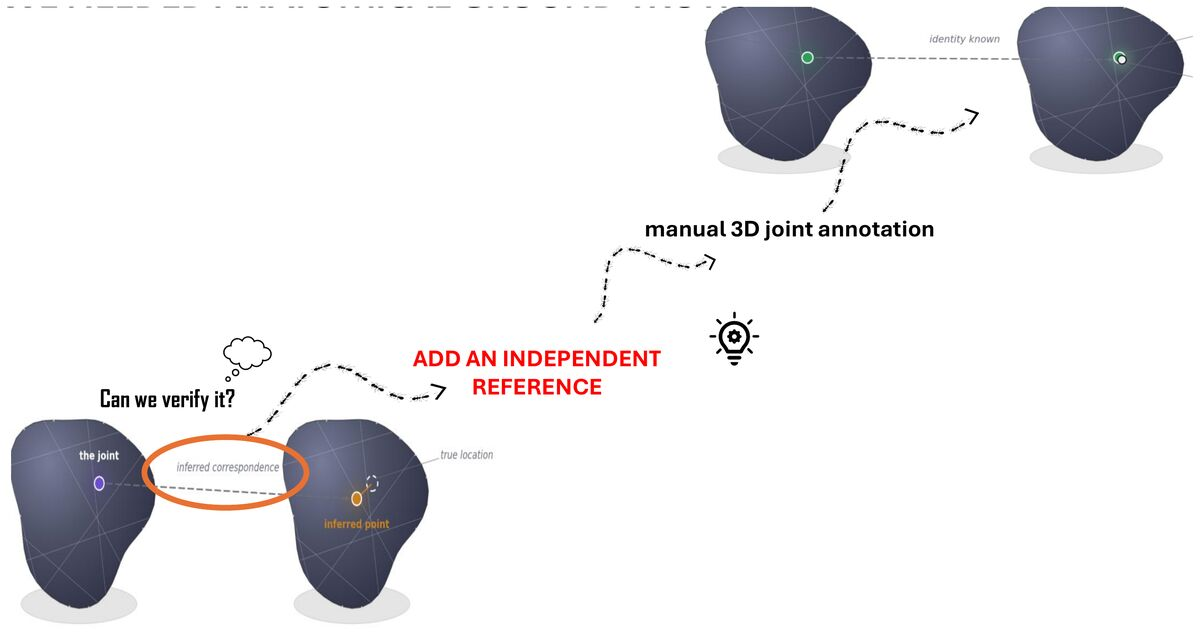
\includegraphics[width=0.34\linewidth]{figures/fig_ground_truth_annotation.jpg}
\caption[Expert joint annotation]{Manual 3D joint annotation as an independent reference,
with identity known by construction, against which the model's inferred correspondence can be
verified and not merely inspected.}
\label{fig:ground-truth}
\end{figure}

\subsection{Scale-dependent validity}
\label{sec:validity-scale}

``The registration is valid'' is therefore not one claim but five, holding at different
scales and supported by different evidence (Table~\ref{tab:validity}). A model can give an
accurate population-level or single-trait measurement while failing to preserve the
individual-level correspondence needed for specimen-by-specimen comparison, and each
statement is supported only at its own level. The expert-supervised fit quantifies the
headroom available; since expert joints are unavailable at inference time, supplying an
equivalent signal automatically is the objective it motivates.

\begin{table}[!htb]
\centering
\caption{Levels of registration validity and the evidence for each.}
\label{tab:validity}
\begin{tabular}{@{}L{0.20\linewidth}L{0.34\linewidth}L{0.34\linewidth}@{}}
\toprule
\textbf{Level} & \textbf{Question} & \textbf{Evidence}\\
\midrule
Geometric agreement & Do the surfaces overlap? & Chamfer, F-score; misleading alone
 (Section~\ref{sec:geometric-agreement})\\
Surface correspondence & Are points mapped geometrically? & Nearest-surface matching;
 label-invariant (Section~\ref{sec:objective})\\
Anatomical correspondence & Does vertex $i$ mark the same structure across specimens? &
 Synthetic oracles, expert benchmark\\
Parametric recovery & Do $\bm\beta,\bm\theta$ mean the same thing across specimens? &
 Region-dependent; nest-mate agreement\\
Measurement validity & Does a derived quantity match a reference? & Head width on 20
 workers; four validity axes\\
\bottomrule
\end{tabular}
\end{table}
